\subsection{Traffic forecasting}
\label{sub:ts_forecasting}
Capturing data about traffic in a highway worth not only for describing its current situation, but also for forecasting future conditions. In this sense, counting the number of cars that have passed for a given point in a given time can be considered as a time series, allowing the use of automatic tools to perform forecasting.

For this work, four methods (three widely used time series forecasters, and one control method) have been used to, automatically, predict the number of cars that will pass in the next period. These methods are included in the forecast package ~\cite{Hyndman08automatictime} of the R program~\cite{R:Bloomfield:2014}, and are the following:

\begin{itemize}
\item {\em Exponential smoothing state space model (ETS)~\cite{ETS:2008}}: Represent a set of methods that decompose the time-series in three different characteristics: error, trend and seasonal, modeling each one with a given equation. The forecasted values are obtained joining the previous equations by addition or multiplication. The corresponding function in the forecast package builds the different models included in the ETS set, and select the one with the best according to the Akaike's Information Criterion (AIC)~\cite{Akaike1973}.
\item {\em ARIMA~\cite{BoxJenk}: This well known method, due to Box and Jenkins } integrates autoregressive (AR) and moving average (MA) models in a three-stage iterative cycle. The phases of every cycle consist of: identifying the time series, estimating of the model's parameters, and verifying the built model. Briefly, every model is defined as a sum of $p+q$ terms. The first $p$  terms are defined by $p$ past values, any of them multiplied by a coefficient; while the last $q$ terms represent the moving averages, also multiplied by their own coefficients.
\item {\em Theta~\cite{Assima2000}}: This univariate forecasting method is based on modifying the local curvature of the time-series, after having applied a second difference to the data. It decomposes the original time series into several modified ones, which are separately extrapolated so that they have to be combined in order to provide the forecasting.
\item {\em Mean}: This is the control method. The future values are computed as the mean of the previous ones.
\end{itemize}

The data used for the experiments are the ones provided by the node 1010 from the PETRA project starting on 12-Oct-2015, 00:00 hours, and finishing on 31-Oct-2015, 23:45 hours, i.e., three entire weeks less one day (there exist no data for November, the first). As data is aggregated every 15 minutes, this means the time-series was composed of $20(days)*24(hours)*4(quarters)=1920$ values.

In order to study the performance of every method, 9 frequently used error measures are shown:
Mean Error ({\em ME}),
 Mean Squared Error ({\em MSE}),
 Root Mean Squared Error ({\em RMSE}),
 Mean Absolute Error ({\em MAE}),
 Mean Absolute Scaled Error ({\em MASE}),
 Median Absolute Error ({\em MdAE}),
 Median Absolute Percentage Error ({\em MdAPE(\%)}),
 Symmetric Mean Absolute Percentage Error ({\em sMAPE(\%)}), and
 Symmetric Median Absolute Percentage Error ({\em sMdAPE(\%)}).
%\begin{itemize}
%\item{\em ME}: Mean Error.
%\item{\em MSE}:  Mean Squared Error.
%\item{\em RMSE}: Root Mean Squared Error.
%\item{\em MAE}: Mean Absolute Error.
%\item{\em MASE}: Mean Absolute Scaled Error.
%\item{\em MdAE}: Median Absolute Error.
%\item{\em MdAPE(\%)}: Median Absolute Percentage Error.
%\item{\em sMAPE(\%)}: Symmetric Mean Absolute Percentage Error.
%\item{\em sMdAPE(\%)}: Symmetric Median Absolute Percentage Error.
%\end{itemize}
Their different features as well as their equations can be found in Hyndman and Koehler's work ~\cite{RePEc:eee:intfor:v:22:y:2006:i:4:p:679-688}

Table ~\ref{tab:forecasting} shows the values for the ten used measures computed over $576$ values, the ones corresponding to the last 6 days (i.e., $30\%$ of the data). The horizon has been set to 1, so that, in order to forecast any given moment all the previous real known data were used to build and train the models and, after this, the next value was forecasted. This way, the problem has been faced as a simulation of what could happen in a continuous system in which new real data where received every 15 minutes so that forecasting models could be also continuously adapted.

As results show, ETS, ARIMA and Theta behave clearly better than the control method. The differences between the three considered methods are, almost nonexistent. In any case, ETS yields the lowest values in six of the measures been used so that, a priori, it could be considered the best candidate to be chosen as the preferred method to forecast this kind of time-series. Figure \ref{fig:forecasted-values} depicts the values forecasted by ETS comparing them with the expected ones.

\begin{table}
\centering
\resizebox{12cm}{!}{
\begin{tabular}{|c|c|c|c|c|c|c|c|c|c|c|}
\hline
ME &MSE &RMSE &MAE &MPE &MAPE &MASE &MdAE &MdAPE & SMAPE(%) & SMdAPE(%) \\
$12.19$ & $9152.5$ & $95.67$ & $84.68$ & $8.17$ & $187.89$ & $4.72$ & $90.76$ & $50.01$ & $69.23$ & $54.87$ \\
\bf{$0.11$} & \bf{$635.11$} & \bf{$25.2$} & \bf{$18.16$} & \bf{$-3.44$} & \bf{$18.71$} & \bf{$1.01$} & \bf{$11.5$} & \bf{$12.64$} & \bf{$17.73$} & \bf{$12.59$} \\
$0.86$ & $662.81$ & $25.75$ & $19.41$ & $4.24$ & $24.51$ & $1.08$ & $15.99$ & $13.82$ & $20.06$ & $14.66$ \\
$0.23$ & $669.3$ & $25.87$ & $19.01$ & $-2.05$ & $20.11$ & $1.06$ & $13.9$ & $13.72$ & $18.57$ & $13.15$ \\

ME &MSE &RMSE &MAE &MPE &MAPE &MASE &MdAE &MdAPE & SMAPE(%) & SMdAPE(%) \\
$1.22$ & $6178.45$ & $78.6$ & $67.75$ & $1.17$ & $198.68$ & $5.34$ & $69.04$ & $58.18$ & $75.77$ & $69.98$ \\
\bf{$0.03$} & $255.64$ & $15.99$ & $11.73$ & \bf{$-3.7$} & \bf{$18.3$} & $0.92$ & $9.21$ & $12.38$ & $17.2$ & $12.53$ \\
$0.13$ & \bf{$245.38$} & \bf{$15.66$} & \bf{$11.5$} & $2.49$ & $19.28$ & \bf{$0.91$} & $9.4$ & \bf{$11.28$} & \bf{$16.17$} & \bf{$11.36$} \\
$0.24$ & $295.8$ & $17.2$ & $12.67$ & $-1.83$ & $19.76$ & $1$ & \bf{$9.06$} & $14.02$ & $18.03$ & $13.82$ \\

ME &MSE &RMSE &MAE &MPE &MAPE &MASE &MdAE &MdAPE & SMAPE(%) & SMdAPE(%) \\
\bf{$-4.07$} & $1352.47$ & $36.78$ & $30.39$ & \bf{$-10.55$} & $324.49$ & $3.93$ & $27.67$ & $60.54$ & $82.44$ & $76.61$ \\
$0.07$ & $91.62$ & $9.57$ & $6.95$ & $-9.37$ & \bf{$33.24$} & $0.9$ & $5.04$ & \bf{$18.43$} & $27.24$ & \bf{$18.47$} \\
$-0.19$ & \bf{$89.59$} & \bf{$9.47$} & \bf{$6.92$} & $2.77$ & $42.46$ & \bf{$0.89$} & \bf{$4.92$} & $18.91$ & \bf{$26.97$} & $19.69$ \\
$0.14$ & $102.48$ & $10.12$ & $7.38$ & $-6.32$ & $36.48$ & $0.95$ & $5.38$ & $20.51$ & $28.27$ & $20.76$ \\

ME &MSE &RMSE &MAE &MPE &MAPE &MASE &MdAE &MdAPE & SMAPE(%) & SMdAPE(%) \\
$9.27$ & $13990.68$ & $118.28$ & $99.08$ & $5.86$ & N/A &$5.49$ & $100.03$ & $56.13$ & $76.08$ & $66.78$ \\
\bf{$-0.06$} & $802.93$ & $28.34$ & $17.85$ & \bf{$3.96$} & N/A &$0.99$ & $11.72$ & $12.15$ & \bf{$14.42$} & $11.24$ \\
$0.26$ & \bf{$739.31$} & \bf{$27.19$} & \bf{$17.06$} & $17.61$ & N/A &\bf{$0.95$} & \bf{$10.52$} & \bf{$11.56$} & $16.15$ & \bf{$10.69$} \\
$0.12$ & $789.6$ & $28.1$ & $18.18$ & $38500.8$ & N/A &$1.01$ & $10.88$ & $12.55$ & $21.3$ & $13$ \\

ME &MSE &RMSE &MAE &MPE &MAPE &MASE &MdAE &MdAPE & SMAPE(%) & SMdAPE(%) \\
$11.05$ & $1493.67$ & $38.65$ & $33.09$ & $19.74$ & N/A &$3.78$ & $33.65$ & $60.83$ & $79.85$ & $61.23$ \\
$0.21$ & $173.88$ & $13.19$ & \bf{$9.56$} & \bf{$-4.66$} & N/A\bf{$1.09$} & \bf{$7.02$} & $21.66$ & \bf{$33.16$} & $22.58$ \\
$2.01$ & \bf{$172.23$} & \bf{$13.12$} & $9.95$ & $9.32$ & N/A$1.14$ & $7.96$ & \bf{$21.61$} & $36.94$ & \bf{$22.51$} \\
\bf{$0.19$} & $180.75$ & $13.44$ & $9.85$ & $-2.72$ & N/A$1.12$ & $7.33$ & $23.25$ & $33.88$ & $23.12$ \\
\hline
\end{tabular}
}
\caption{Forecasting.}
\label{tab:forecasting}
\end{table}

\begin{figure}[!ht]
	\begin{center}
		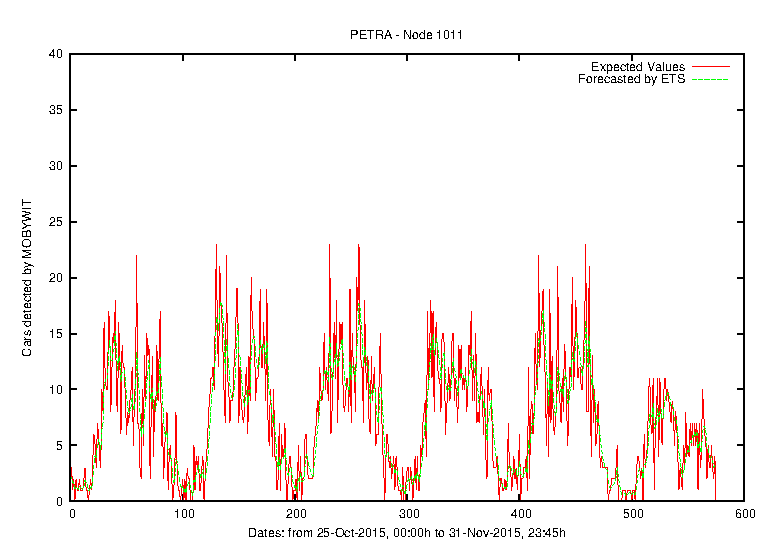
\includegraphics[width=14cm]{imgs/PETRA/forecasting-PETRA-1011.eps}
		\caption{Expected vs forecasted number of cars in node 1011, according to MOBYWIT's records. Forecasted values are provided by smoothing state space model (ETS). }
		\label{fig:forecasted-values}
	\end{center}
\end{figure}



%% ---------------------- REFERENCIAS que he de copiar a mobility.bib
